% %%%%%%%%%%%%%%%%%%%%%%%%%%%%%%%%%%%%%%%%%%%%%%%%%%%%%%%%%%%%%%%%%%%%%%%%%%%%%%%%%%%%%%%
% Appendices
% Statistics
% %%%%%%%%%%%%%%%%%%%%%%%%%%%%%%%%%%%%%%%%%%%%%%%%%%%%%%%%%%%%%%%%%%%%%%%%%%%%%%%%%%%%%%%

\section{Thesis Statistics}
\label{app:stats}

\lettrine{T}{o} provide insight into the scope and duration of this thesis work, we present statistics and key information in this appendix.
The work spanned multiple repositories managed through Git version control.

During the first year and a half, extensive exploration was conducted using Python scripts, culminating in the Python model. This work was maintained in the \textit{Python Script} repository.
The second half focused on the \acrshort{rtl} implementation, distributed across several repositories: \textit{SpDCache RTL} containing the core \acrshort{rtl} implementation, \textit{CVA6 RTL} with modifications to the CVA6 RISC-V core for \acrlong{spdc}'s new instructions, \textit{RTL Platform} providing the compilation and simulation environment, and \textit{Software} containing C programs for the \acrlong{op} \acrshort{spmv} kernel.
In parallel, the \textit{Benchmarks} repository was developed for efficient benchmarking and performance evaluation, contributed by student Jules DUBOIS during an internship.

Throughout the thesis, several publications were produced: a state-of-the-art survey~[\ref{publ:SoA}], a paper on initial \acrlong{spdc} results~[\ref{publ:SpDC}], a patent covering the development concepts around \acrlong{spdc}~[\ref{publ:patent}], a paper on the \acrshort{rtl} implementation and analytical model (currently under resubmission), and this manuscript.
Figure~\ref{fig:app:stats:commits} illustrates the timeline of all commits across each repository.

\begin{figure}[htbp]
    \centering
    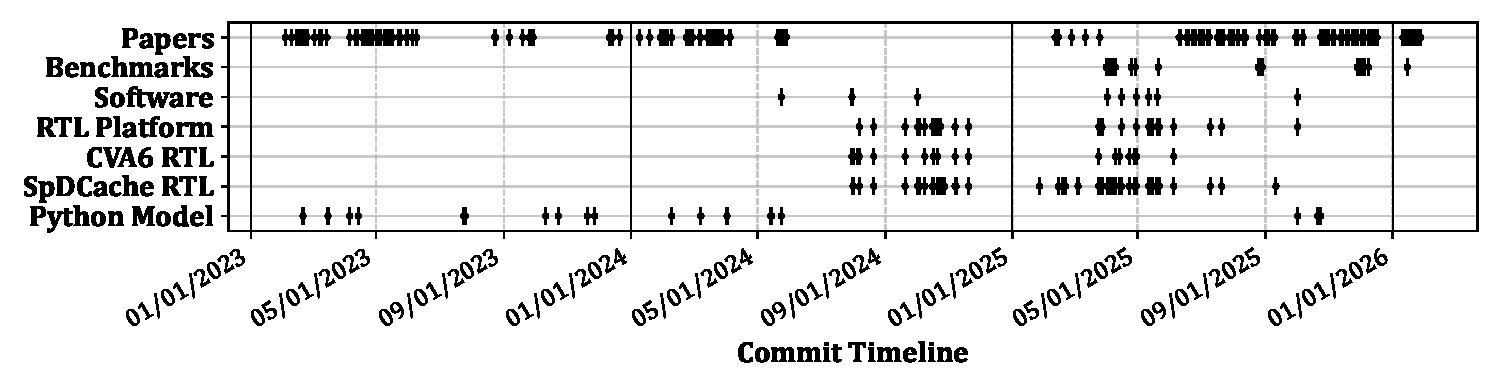
\includegraphics[width=\linewidth]{PreAndPostSections/Figures/PDF/Stats_Commits.pdf}
    \caption{Timeline of Commits Across All Working Repositories and Publications}
    \label{fig:app:stats:commits}
\end{figure}

To provide a sense of the work delivered, we present the number of new lines of code for each repository (excluding papers) after final modifications:
\begin{itemize}
    \item \textit{Python Scripts}: 18,590 lines;
    \item \textit{SpDCache RTL}: 5808 lines (33,696 $\to$ 39,504 total);
    \item \textit{CVA6 RTL}: 255 lines (36,623 $\to$ 36,878 total);
    \item \textit{RTL Platform}: 56 lines (6156 $\to$ 6212 total);
    \item \textit{Software}: 1554 lines;
    \item \textit{Benchmarks}: 7642 lines.
\end{itemize}
Additionally, Figure~\ref{fig:app:stats:languages} shows the programming language distribution across each repository.

\begin{figure}[htbp]
    \centering
    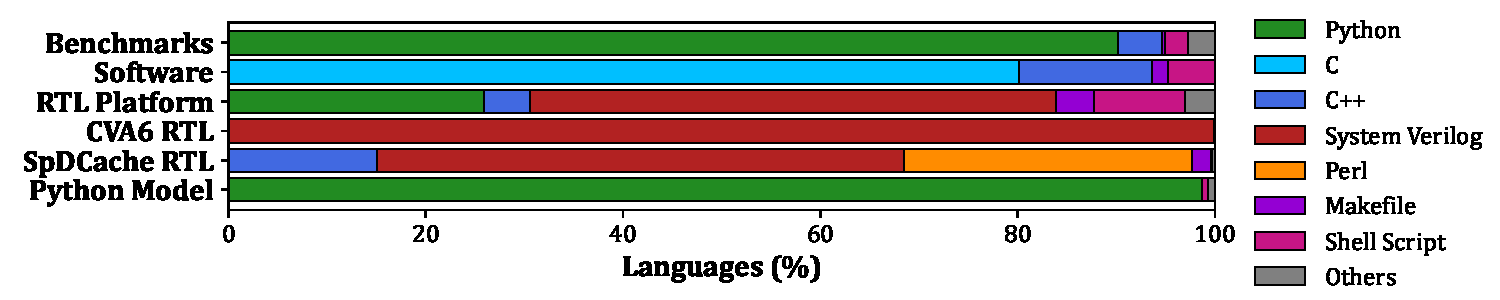
\includegraphics[width=\linewidth]{PreAndPostSections/Figures/PDF/Stats_Languages.pdf}
    \caption{Programming Language Distribution Across All Working Repositories}
    \label{fig:app:stats:languages}
\end{figure}